\documentclass[xcolor=dvipsnames,aspectratio=169,t]{beamer}
  % t means frames are vertically centered to the top
\usepackage{slides-header}
\title{Applications of Determinants}

\begin{document}
\maketitle

\begin{frame}{Using Determinants to Solve Systems of Equations}

\[ \begin{array}{rcrcr}
3x_1 & - & 2x_2 & = & \alert{6}\\
-5x_1 & + & 4x_2 & = & \alert{8}\\
\end{array} \]

\bbox
For a square matrix $\dsty A = \begin{bmatrix} \mathbf{a}_1 &  \mathbf{a}_2  & \ldots &  \mathbf{a}_n \end{bmatrix}$ and column vector $\mathbf{b}$, \alert{if we replace the $j^{\mbox{th}}$ column of $A$ with $\mathbf{b}$}, we denote the new matrix
\[ \alert{A_j(\alert{ \mathbf{b}}) } =  A = \begin{bmatrix} \mathbf{a}_1 & \ldots & \mathbf{a}_{j-1} & \alert{\mathbf{b}} & \mathbf{a}_{j+1} & \ldots &   \mathbf{a}_n \end{bmatrix} .\]
\ebox

\pause
Let  $\dsty A = \begin{bmatrix} 3 & -2 \\ -5 & 4 \end{bmatrix}$ and \alert{$\dsty \mathbf{b} = \begin{bmatrix} 6\\ 8 \end{bmatrix}$}. Then

\[ A_1( \mathbf{b}) = \begin{bmatrix} \alert{6} & -2 \\ \alert{8} & 4 \end{bmatrix} \quad \mbox{and} \quad
A_2( \mathbf{b}) = \begin{bmatrix} 3 & \alert{6}  \\ -5 & \alert{8} \end{bmatrix} .\]

\end{frame}

\begin{frame}{Cramer's Rule}
  \bbox
  Let $A$ be an invertible $n \times n$ matrix. For any $\mathbf{b}$ in $\mathbb{R}^n$, the unique solution to $A\x=\b$ is $\x$, where the $j^{\mbox{th}}$ entry of $\x$ is given by

  \[ x_j = \frac{\det \alert{ A_j(\b) }}{\det A} \quad \mbox{for } j=1,2, \ldots, n.\]
  \ebox

  \pause
\begin{columns}[T]

\column{0.25\tw}

\[ \begin{array}{rcrcr}
3x_1 & - & 2x_2 & = & \alert{6}\\
-5x_1 & + & 4x_2 & = & \alert{8}\\
\end{array} \]

\[ \mathbf{x} = \begin{bmatrix} \frac{\alert{40}}{2} \\ \ \\ \frac{\colorb{54}}{2} \end{bmatrix} = \begin{bmatrix} 20 \\ 27 \end{bmatrix} \]

\column{0.25\tw}

\[ A = \begin{bmatrix} 3 & -2 \\ -5 & 4 \end{bmatrix} \]

\[ \det A = 2 \]

\column{0.25\tw}

\[ \alert{A_1( \mathbf{b})} = \begin{bmatrix} \alert{6} & -2 \\ \alert{8} & 4 \end{bmatrix} \]

\[ \alert{\det A_1(\mathbf{b})  = 40} \]

\column{0.25\tw}

\[ \colorb{A_2( \mathbf{b})} = \begin{bmatrix} 3 & \colorb{6}  \\ -5 & \colorb{8} \end{bmatrix} \]

\[ \colorb{\det A_2(\mathbf{b})  = 54} \]

\end{columns}
\end{frame}

\begin{frame}{Proof of Cramer's Rule}
  \bbox
  The unique solution to $A\x=\b$ is $\x$, where the  $\displaystyle x_j = \frac{\det \alert{ A_j(\b)}}{\det A}$.
  \ebox

  \pause
  {\small
  \begin{proof}
  Let $\dsty A = \begin{bmatrix} \mathbf{a}_1 &  \mathbf{a}_2  & \ldots &  \mathbf{a}_n \end{bmatrix}$ be an invertible $n \times n$ matrix, where each $\mathbf{a}_i$ denotes a column vector of $A$. Let $\mathbf{x}$ be the unique solution to the equation \colorb{$A \mathbf{x} = \mathbf{b}$}. We denote
  $\dsty \alert{I_j(\mathbf{x})} = \begin{bmatrix} \mathbf{e}_1 & \ldots &  \mathbf{e}_{j-1}  & \mathbf{x} & \mathbf{e}_{j+1} & \ldots & \mathbf{e}_n \end{bmatrix}$,
  and consider the product

  \begin{columns}[T]

  \column{0.65\tw}

  \begin{align*}
  A \alert{I_j(\x)} &= A  \begin{bmatrix} \mathbf{e}_1 & \ldots &  \mathbf{e}_{j-1}  & \x & \mathbf{e}_{j+1} & \ldots & \mathbf{e}_n \end{bmatrix} \\
  &= \begin{bmatrix} A\mathbf{e}_1 & \ldots &  A\mathbf{e}_{j-1}  & \colorb{A\x} & A\mathbf{e}_{j+1} & \ldots & A\mathbf{e}_n \end{bmatrix} \\
  &=  \begin{bmatrix} \a_1 &  \ldots & \a_{j-1} &  \colorb{\b}  & \a_{j+1} & \ldots &  \a_n \end{bmatrix} = A_j (\b).
  \end{align*}
  
  \pause
  Using the multiplicative property of determinants, we have

  \column{0.35\tw}

  \begin{align*}
  & \det A_j ( \b )  = \det \left( A I_j(\x) \right)\\
  &= \left( \det A \right) \left( \det I_j(\x) \right) = \left( \det A \right) x_j.
  \end{align*}
  Therefore, we have $\dsty x_j = \frac{ \det A_j ( \b )}{\det A}$.
  \end{columns}

  \end{proof}}
\end{frame}


\begin{frame}{Formula for the Inverse of a Matrix}
  \medskip
  
  If $A = \begin{bmatrix} a & b \\ c & d \end{bmatrix}$, then
  $A^{-1} = \displaystyle\frac{1}{\blue{ad-bc}} \begin{bmatrix} d & -b \\ -c & a \end{bmatrix}$,
  when $\blue{\det A = ad-bc} \ne 0$.
  \bigskip
  
  \qquad Is there a similar formula for $A^{-1}$ for \alert{larger matrices}?
  \vspace*{2em}
  
  \pause
  Let $A$ be an $n\times n$ matrix.
  The \alert{adjugate $\adj A$} of $A$ (also called \emph{classical adjoint}) is defined by
  \bigskip
  
  \begin{columns}
  
  \column[T]{.5\textwidth}
  $\adj A =
  \begin{bmatrix}
    C_{11} & C_{21} & \ldots & C_{i1} & \ldots & C_{n1} \\
    C_{12} & C_{22} & \ldots & C_{i2} & \ldots & C_{n2} \\
    \vdots & \vdots & \ddots & \vdots &        & \vdots \\
    C_{1i} & C_{2i} & \ldots & \red{C_{ji}} & \ldots & C_{ni} \\
    \vdots & \vdots &        & \vdots & \ddots & \vdots \\
    C_{1n} & C_{2n} & \ldots & C_{jn} & \ldots & C_{nn}
  \end{bmatrix}
  $,
  
  \column[T]{.5\textwidth}
  \bigskip
  
  where the \alert{cofactor} $\alert{C_{ij}}=(-1)^{i+j} \det A_{ij}$.
  \vspace*{1.5em}
  
  Note the \alert{reversed indices!!!}
  \medskip
  
  The adjugate is the \blue{transpose} 
  
  \quad of the matrix of cofactors.
  
  \end{columns}
\end{frame}


\begin{frame}{Formula for the Inverse of a Matrix}
  \bbox
    Let $A$ be an invertible $n\times n$ matrix.
    Then $A^{-1} = \displaystyle\frac{1}{\det A} \  \adj A$.
  \ebox
  
  \pause
  \blue{\large Proof 1.}
  
  Let $D=\alert{A^{-1}}$.  Then $AD=I$.  To find the $j$th column $\d_j$ of $D$, we solve $A\d_j=\e_j$.
  
  To find the $i$th entry of $\d_j$, we apply \blue{Cramer's Rule}:
  \begin{align*}
    \text{$i$th entry of $\d_j$} 
    = \frac{\det A_i(\e_j)}{\det A}
    &= \textstyle \frac{1}{\det A} \det \begin{bmatrix} \a_1 & \ldots & \a_{i-1} & \e_j & \a_{i+1} & \ldots & \a_n \end{bmatrix} \\
    &= \textstyle \frac{1}{\det A} (-1)^{j+i} \det A_{ji} \quad \text{by expanding about column $i$}\\
    &= \textstyle \frac{1}{\det A} \alert{C_{ji}}.
  \end{align*}
  Hence, the $ij$th entry of $A^{-1}$ is $\textstyle \frac{1}{\det A} \alert{C_{ji}}$.
\end{frame}


\begin{frame}{Formula for the Inverse of a Matrix}
  \bbox
    Let $A$ be an invertible $n\times n$ matrix.
    Then $A^{-1} = \displaystyle\frac{1}{\det A} \  \adj A$.
  \ebox
  
  \pause
  \blue{\large Proof 2.}
  
  We show that \blue{$A \, (\adj A) = (\det A) I_n$}.
  
  The $i,j$ entry of $A \, (\adj A)$ is 
  $\displaystyle
    \sum_{k=1}^n \red{a_{ik}} (\adj A)_{kj}
   =\sum_{k=1}^n \red{a_{ik}} C_{jk}.
   =\sum_{k=1}^n \red{a_{ik}} (-1)^{j+k} \det A_{jk}$.
  \medskip
  
  \pause
  This is the determinant of $A$ after replacing the $j$th row with the \red{$i$th row}, which is:
  \medskip
  
  \hspace*{6em} $\alert{\det A}$, if $i=j$; \qquad \blue{$0$}, if $i\ne j$ (since there is a repeated row).
  \vspace*{1.5em}
  
  \pause
  Since $A$ is invertible, $\alert{A^{-1}} A \, (\adj A) = \alert{A^{-1}} (\det A) I_n$.
  Thus, \blue{$A^{-1} = \displaystyle\frac{1}{\det A} \  \adj A$}.
\end{frame}


\begin{frame}{Example}
  \medskip
  
  Compute the inverse of
  $A=\begin{bmatrix} 1 & 0 & 3 \\ 0 & -2 & -2\\ 1 & -3 & 1 \end{bmatrix}$.
  \bigskip
  
  \pause
  $\alert{\det A} = \red{-2 + 0 + 0} \ \blue{+6 -6 -0} = -2$.
  \bigskip
  
  \begin{columns}
  \column[T]{.3\textwidth}
  \pause
  $\alert{\adj A} = 
    \begin{bmatrix} -8 & -9 & 6 \\ \alert{-2} & -2 & 2 \\ 2 & 3 & -2 \end{bmatrix}
  $.
  
  \column[T]{.6\textwidth}
  \pause\vspace*{-1em}
  \begin{align*}
      \alert{(\adj A)_{21}} = C_{12} &= (-1)^{1+2} \det A_{12} \\ 
                                     &= (-1)^3 [0\cdot 1 - 1\cdot (-2)] = -2.
  \end{align*}
  \end{columns}
  \vspace*{2.5em}
  
  \[
    \alert{A^{-1}} = \frac{1}{\det A} \ \adj A 
    = \frac{1}{-2} \begin{bmatrix} -8 & -9 & 6 \\ -2 & -2 & 2 \\ 2 & 3 & -2 \end{bmatrix}
    = \begin{bmatrix} 4 & 9/2 & -3 \\ 1 & 1 & -1 \\ -1 & -3/2 & 1 \end{bmatrix}.
  \]
\end{frame}


\begin{frame}{}
\vspace*{7em}

\begin{center}
{\Huge \blue{\textbf{Volumes}}}
\end{center}
\end{frame}



\begin{frame}{Volume of 2d Parallelogram}
\bigskip
  
  Let $A=\begin{bmatrix} a & b \\ c & d \end{bmatrix}$.  Let $\mathbf{u}=(a,b)$ and $\mathbf{v}=(c,d)$.
  \medskip
  
  The origin, $\mathbf{u}$, $\mathbf{v}$, and $\mathbf{u}+\mathbf{v}$ form a \alert{parallelogram $\mathcal{P}$}.
  
  \pause
  \begin{theorem}
    The area of the parallelogram $\mathcal{P}$ in $\mathbb{R}^2$ is $|\det(A)|$.
  \end{theorem}

  \url{https://www.desmos.com/calculator/iksjsllpxz}
  
  \pause
  Proof sketch:
  \begin{enumerate}
    \item Rotate the parallelogram so that $\mathbf{u}$ is on the positive $x$-axis.
    \item Flip the parallelogram (if necessary) so that $\mathbf{v}$ is above the $x$-axis.
    \item Horizontally scale the parallelogram so that $\mathbf{u}=(1,0)$.
    \item Horizontally shear the parallelogram so that $\mathbf{v}$ is on the $y$-axis.
    \item Vertically scale the parallelogram so that $\mathbf{v}=(0,1)$.
  \end{enumerate}
\end{frame}

\begin{frame}{Volume of 3d Parallelopiped}
\medskip

  Three vectors $\mathbf{u}$, $\mathbf{v}$, and $\mathbf{w}$ in $\mathbb{R}^3$ form a \alert{parallelopiped} with vertices \\
  $\qquad \mathbf{0},
  \mathbf{u},\mathbf{v},\mathbf{w},
  \mathbf{u}+\mathbf{v},\mathbf{u}+\mathbf{w},\mathbf{v}+\mathbf{w},
  \mathbf{u}+\mathbf{v}+\mathbf{w}$.
  \bigskip

  \url{https://www.geogebra.org/m/VvR6MeR5}
  \bigskip
  
  \pause
  \begin{theorem}
    The volume of the parallelopiped $\mathcal{P}$ in $\mathbb{R}^3$ is $|\det(A)|$, where $A$ has rows $\mathbf{u}$, $\mathbf{v}$, and $\mathbf{w}$.
  \end{theorem}
  \bigskip
  
  This works in higher dimensions: for an $n\times n$ matrix $A$, the volume of the \alert{parallelotope} in $\mathbb{R}^n$ corresponding to the rows of $A$ is given by $|\det(A)|$.
    
\end{frame}

\begin{frame}{Linear Transformations}
\bigskip
  
  Let $T\colon \mathbb{R}^n \to \mathbb{R}^n$ be a linear transformation 
  where $\mathbf{x} \mapsto A \mathbf{x}$.
  
  Consider the unit parallelotope $\mathcal{U}$ with volume $1$ determined by the origin and $\mathbf{e}_1,\mathbf{e}_2,\dots,\mathbf{e}_n$.
  \smallskip
  
  What is the \alert{volume} of $T(\mathcal{U})$?
  \bigskip
  
  \pause
  $T(\mathcal{U})$ is a parallelotope determined by the columns of $A I = A$.
  So its volume is $\alert{|\det A|}$.
  
  \vspace*{2em}
  
  \pause
  Since $T$ is a linear transformation, the volume of \alert{any shape} is scaled by $|\det A|$,
  \smallskip
  
  \quad ie, if $\mathcal{R}$ is a shape in $\mathbb{R}^n$ with volume $\alert{r}$,
  then $T(\mathcal{R})$ has volume \alert{$|\det A|r$}.
    
\end{frame}


\begin{frame}{Example: Area of an Ellipse}
  \medskip
  
  Let $T\colon \R^2 \to \R^2$ be a linear transformation, with associated matrix $A$.
  
  The image of the \blue{unit circle} centered at the origin is an \alert{ellipse}.
  What is the \alert{area} of the ellipse?
  \vspace*{2em}
  
  \begin{columns}[T]
  \column[T]{.5\textwidth}
  \vspace*{-9em}%  % FIXME: Need to figure out how to correctly place images.
  \hspace*{-2.5em}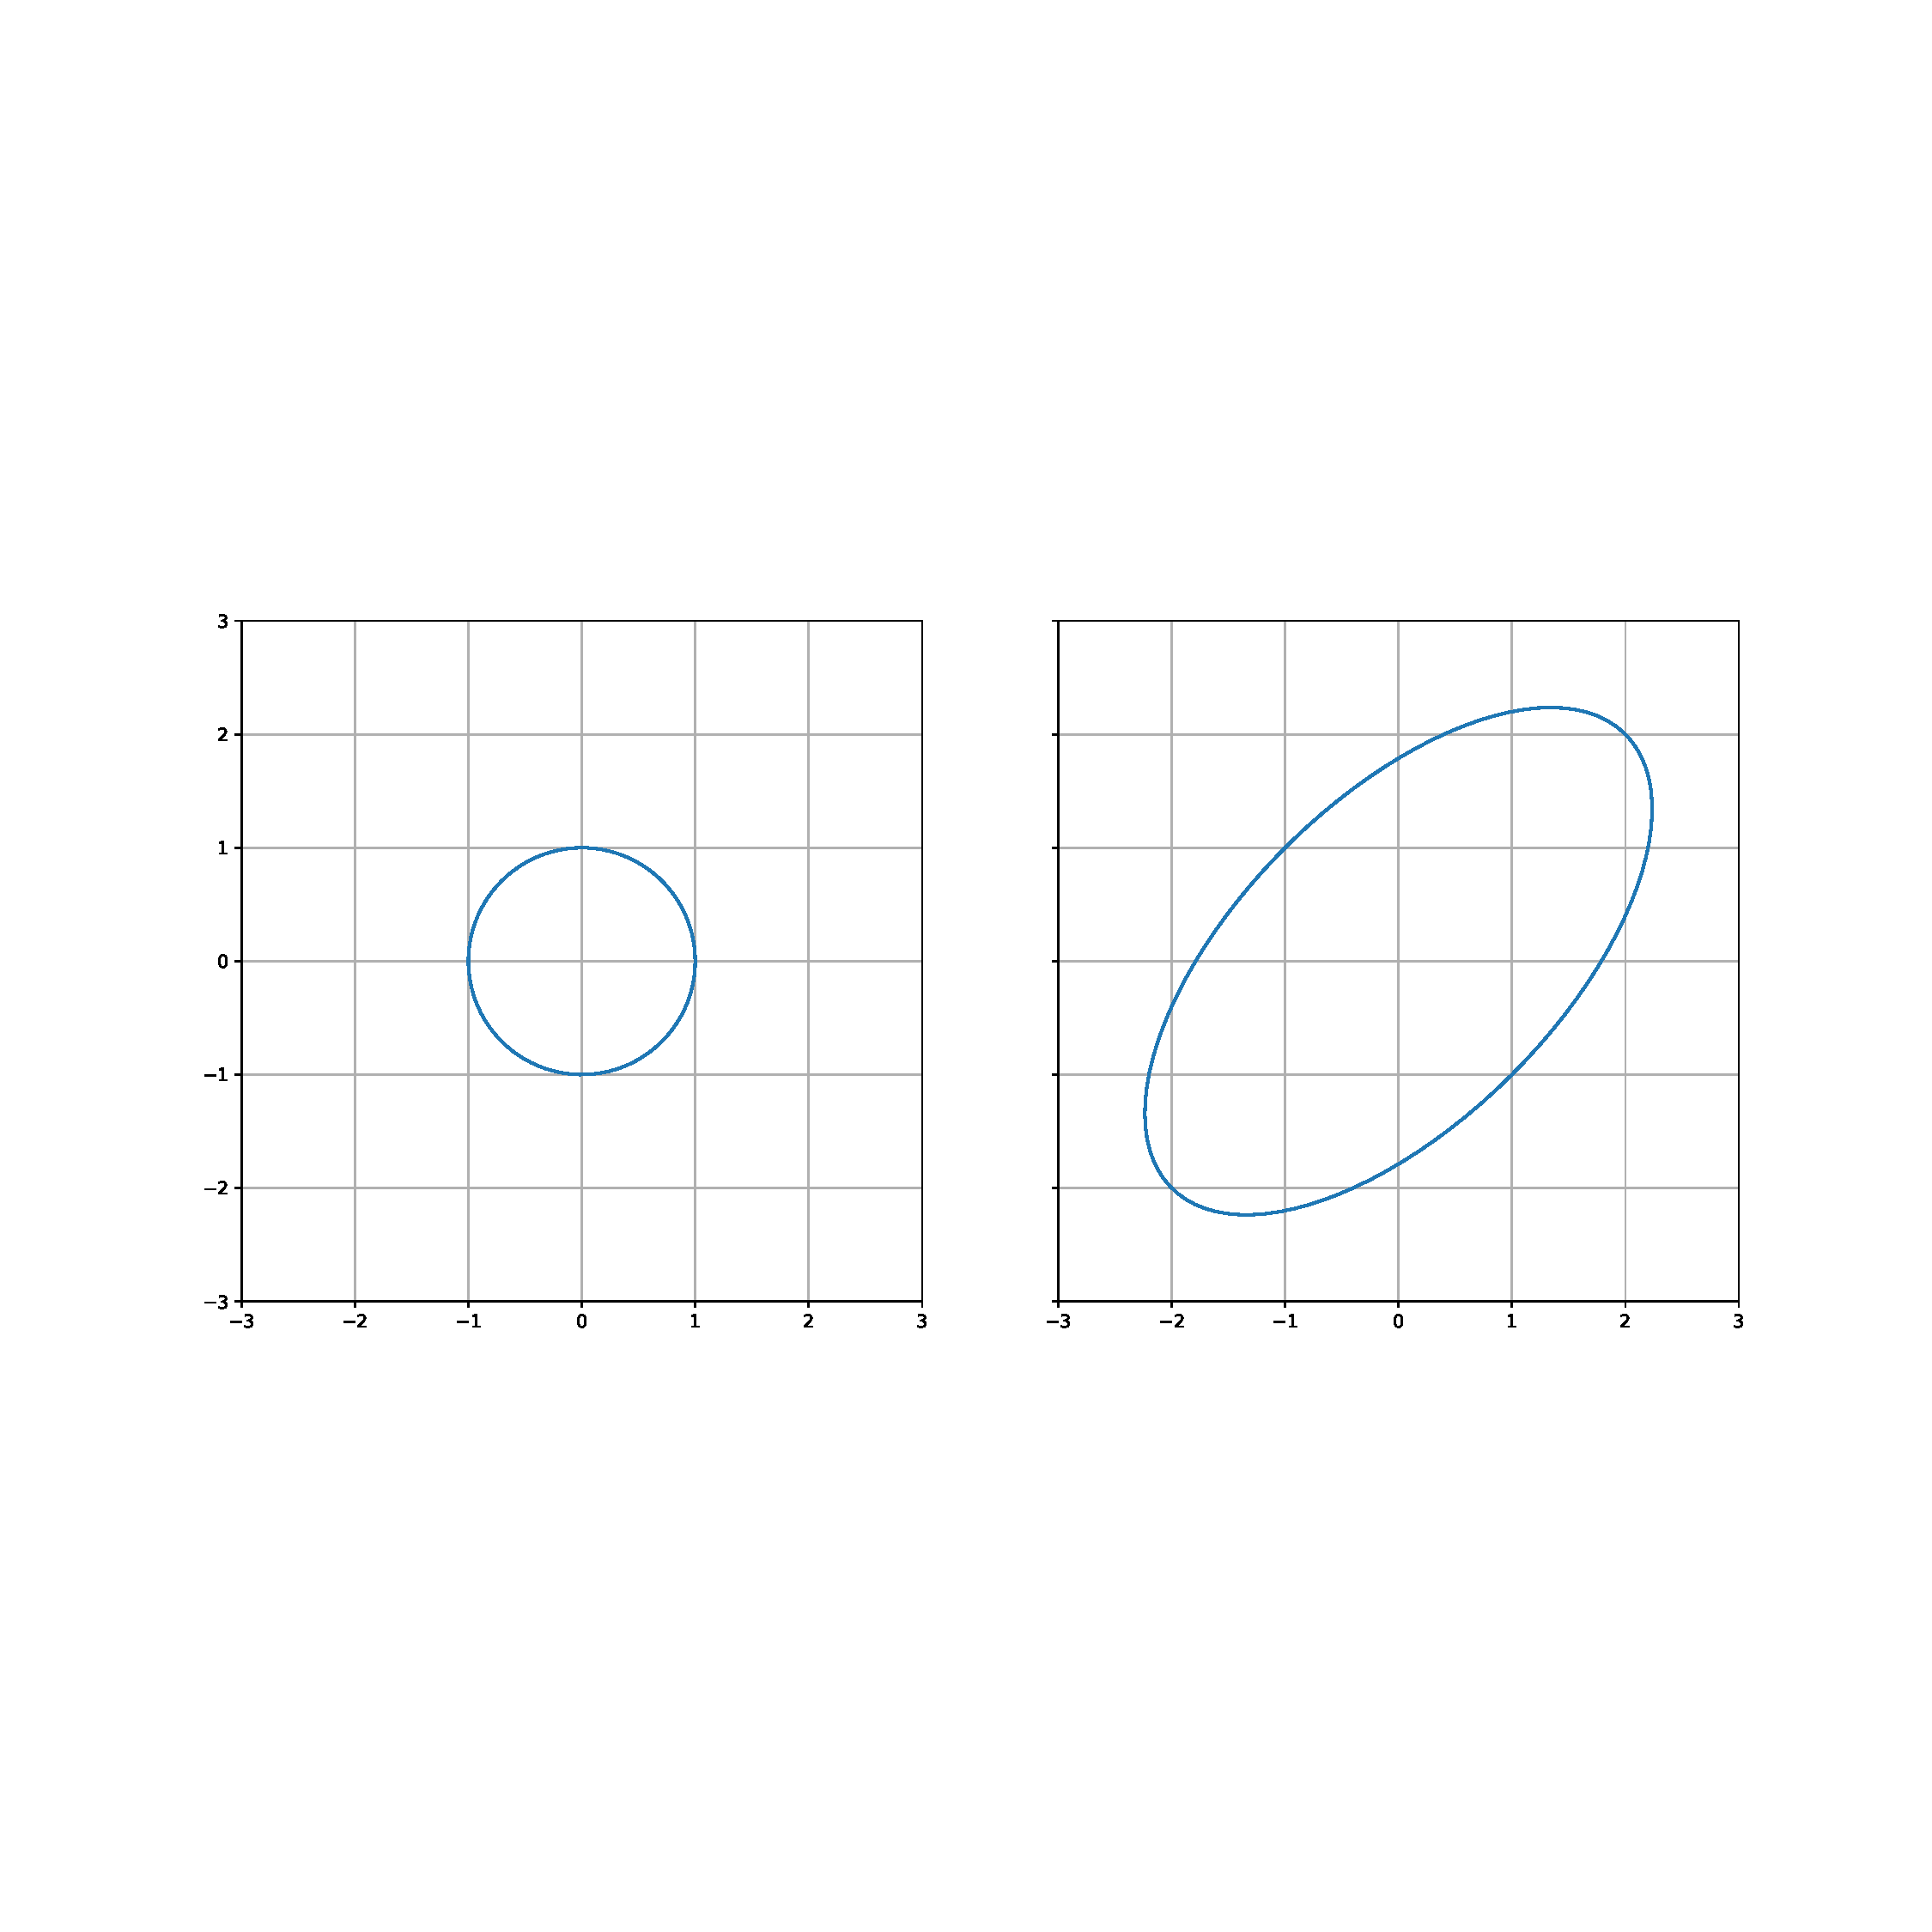
\includegraphics[scale=.25]{images/ellipse.pdf}%
  
  \column[T]{.45\textwidth}
  $A=\begin{bmatrix} 1 & 2 \\ -1 & 2 \end{bmatrix}$.
  \bigskip
  
  \pause
  The area of the \blue{unit circle} is $\pi r^2 = \pi$.
  \medskip
  
  The area of the \alert{ellipse} is $|\det A| \pi = 4\pi$.
  \end{columns}

  
  
\end{frame}


\begin{frame}{Change of Variable in Integration}
  \bigskip
  
  Consider the integral \colorb{$\displaystyle\int f(x) \ dx$}, and a change of variables \colorr{$x=g(u)$}.
  \bigskip
  
  \pause
  \qquad Then $\displaystyle \colorb{\int f(x) \ dx}= \int f(\colorr{g(u)}) \ \colorr{g'(u) du}$.
  \vspace*{1.5em}
  
  \pause
  Consider $\displaystyle\colorb{\int_a^b f(x) \ dx}=\int_4^9 \sqrt{x} \ dx$.
  Let $\alert{x=u^2}$.
  \medskip
  
  \quad Then $=\displaystyle \int_{\sqrt{4}}^{\sqrt{9}} \sqrt{\colorr{u^2}} \ \colorr{2u \ du}
              = \int_{2}^{3} 2u^2 \ du
              = \left. \frac{2}{3}u^3 \right|_{2}^{3}
              = \frac{2}{3}\left(3^3 - 2^3\right) = \frac{38}{3}.$
\end{frame}

\begin{frame}{Change of Variable in Integration}
  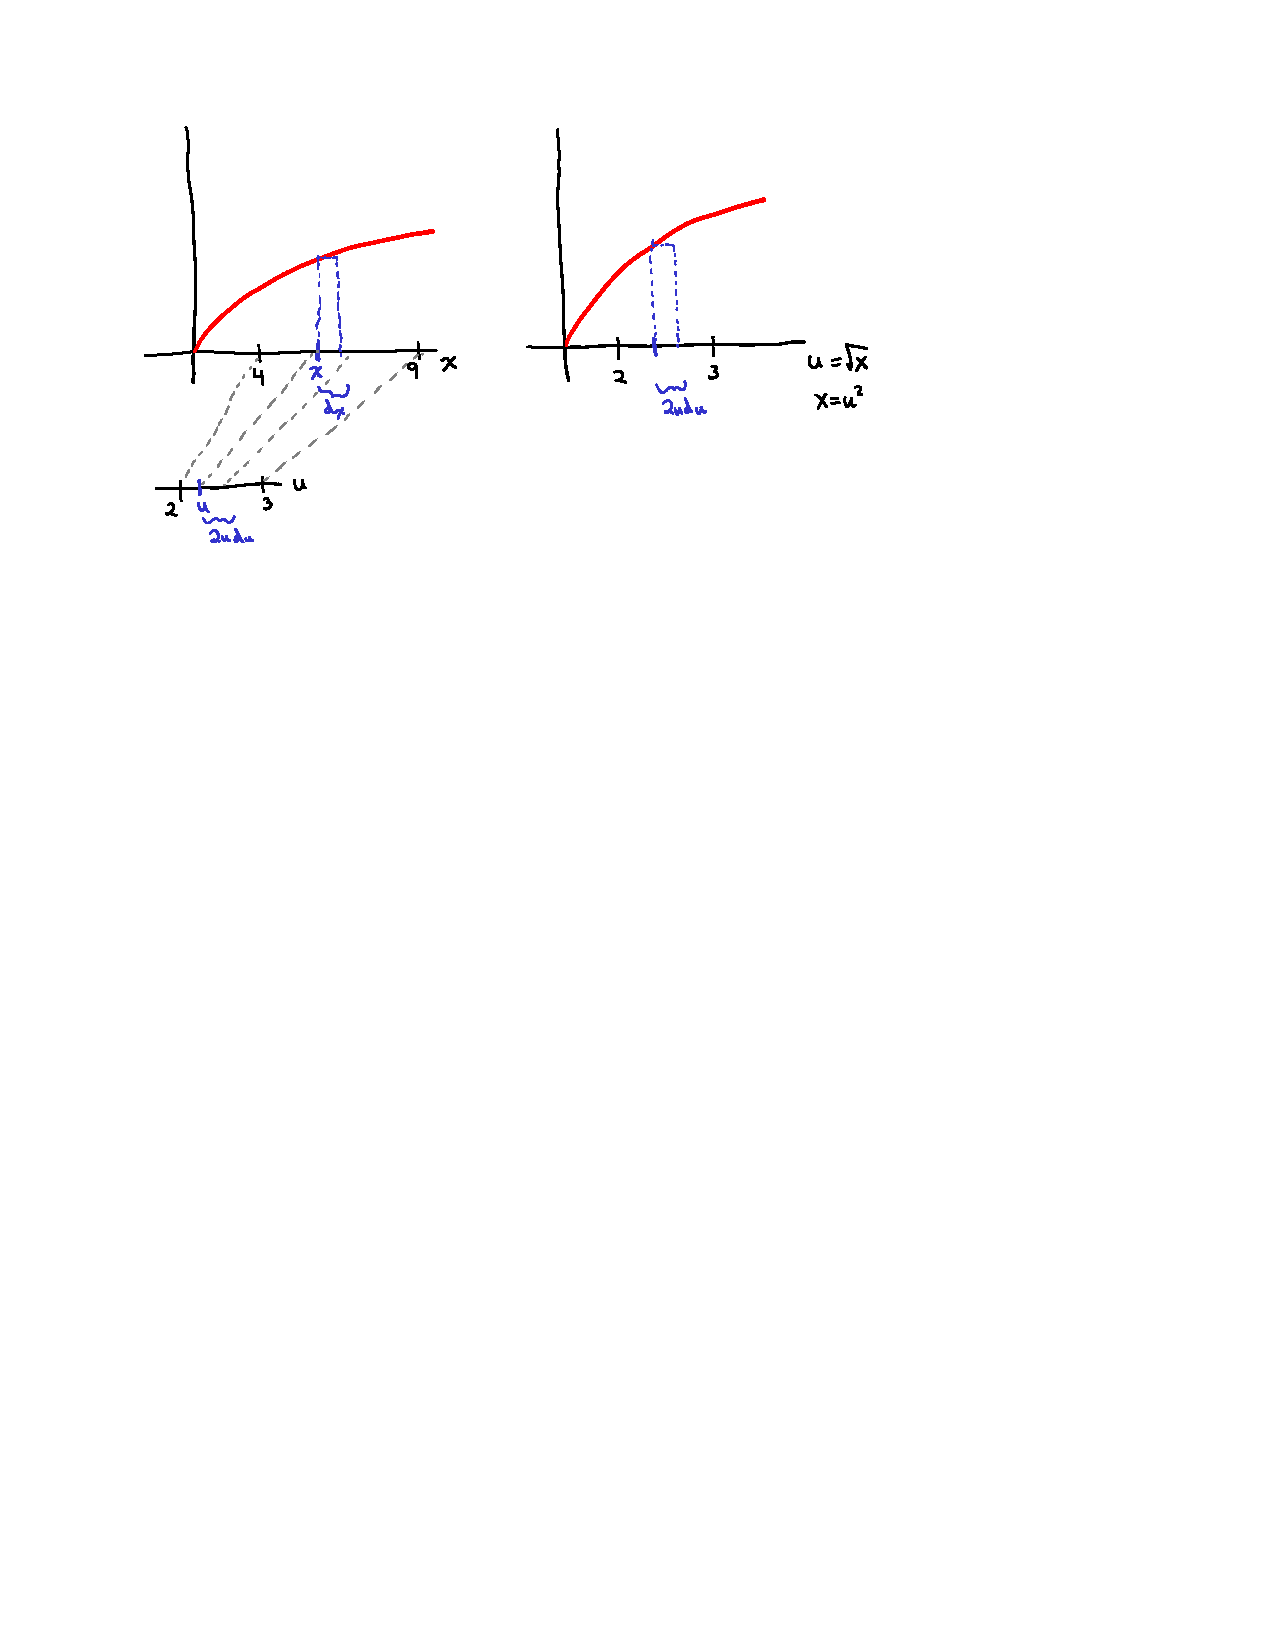
\includegraphics[clip,trim=1cm 0 0 5em]{images/ChangeOfVar.pdf}  % left lower right upper
\end{frame}

\begin{frame}{Polar Coordinates in 2 dimensions}
  \bigskip
  
  Consider the integral \colorb{$\displaystyle\iint f(x,y) \ dx\, dy$}, 
  and a change of variables $\displaystyle\colorr{{x=r \cos \theta} \atop {y=r \sin \theta}}$.
  \smallskip
  
  \url{https://www.desmos.com/calculator/bfn2hgtvqp}
  \medskip
  
  \pause
  The correction needed describes how the area of a little rectangle $dx \times dy$ changes with respect to $r$ and $\theta$, and is given by the determinant of the \alert{Jacobian matrix}:
  \[
    \displaystyle
    \mathbf{J}(r,\theta)
      =\begin{bmatrix}
        \frac{\partial x}{\partial r} & \frac{\partial x}{\partial \theta} \smallskip\\
        \frac{\partial y}{\partial r} & \frac{\partial y}{\partial \theta}
       \end{bmatrix}
      =\begin{bmatrix}
        \cos \theta & -r \sin\theta \\
        \sin \theta &  r \cos\theta
       \end{bmatrix}
  \]

  \pause
  \begin{align*}
    \text{Then } \colorb{\iint f(x,y) \ dx\,dy}
      &=\iint f(\colorr{r\cos\theta,r\sin\theta}) \ \colorr{\det \mathbf{J}\ dr\, d\theta} \\
      &=\iint f(\colorr{r\cos\theta,r\sin\theta}) \ \colorr{r \ dr\, d\theta}.
  \end{align*}
\end{frame}

\begin{frame}{Spherical Coordinates in 3 dimensions}
  \bigskip
  
  \def\phi{\varphi}  % making phi more scripty
  
  Consider the integral \colorb{$\displaystyle\iiint f(x,y,z) \ dx\, dy\, dz$}, 
  and a change of variables $\colorr{\substack{x=\rho \sin\phi \cos\theta \\ y=\rho \sin\phi \sin\theta \\ z = \rho \cos\phi}}$.
  \medskip
  
  \url{https://www.geogebra.org/m/h9xS5ZZs}
  \medskip
  
  \pause
  \[
    \displaystyle
    \mathbf{J}(r,\theta)
      =\begin{bmatrix}
        \frac{\partial x}{\partial \rho} & \frac{\partial x}{\partial \phi} & \frac{\partial x}{\partial \theta} \smallskip\\
        \frac{\partial y}{\partial \rho} & \frac{\partial y}{\partial \phi} & \frac{\partial y}{\partial \theta} \smallskip\\
        \frac{\partial z}{\partial \rho} & \frac{\partial z}{\partial \phi} & \frac{\partial z}{\partial \theta}
       \end{bmatrix}
      =\begin{bmatrix}
        \sin\phi \cos\theta & \rho \cos\phi \cos\theta & -\rho \sin\phi \sin\theta \\
        \sin\phi \sin\theta & \rho \cos\phi \sin\theta &  \rho \sin\phi \cos\theta \\
        \cos\phi            &-\rho \sin\phi            &  0
       \end{bmatrix}
  \]
  \pause
  \begin{align*}
    \text{Then } \colorb{\iiint f(x,y,z) \ dx\,dy\,dz}
      =\iiint f(\colorr{x,y,z}) \ \colorr{\det \mathbf{J}\ d\rho\, d\phi\, d\theta} \\
      =\iiint f(\colorr{\rho \sin\phi \cos\theta,\rho \sin\phi \sin\theta,\rho \cos\phi}) \ \colorr{\rho^2 \sin\phi \ d\rho\, d\phi\, d\theta}.
  \end{align*}
\end{frame}


\end{document}

Beautiful, but phi and theta symbols are switched:
https://www.geogebra.org/m/FzkZPN3K

https://www.desmos.com/calculator/b0tulhgt9l

https://en.wikipedia.org/wiki/Spherical_coordinate_system

https://en.wikipedia.org/wiki/Jacobian_matrix_and_determinant#Example_2:_polar-Cartesian_transformation
